\documentclass[10pt,xcolor=dvipsnames]{beamer}

\usepackage{graphicx,subfigure,url}

\def\bfc{\mathbf{c}}
\def\bfx{\mathbf{x}}
\def\bbP{\mathbb{P}}
\def\cH{\mathcal{H}}
\def\cY{\mathcal{Y}}
\def\cL{\mathcal{L}}

\usepackage{listings}
\lstset{basicstyle=\footnotesize\ttfamily,breaklines=true}

% example themes
\usetheme{Frankfurt}
\usecolortheme{seahorse}
\usecolortheme{rose}

% put page numbers
% \setbeamertemplate{footline}[frame number]{}
% remove navigation symbols
% \setbeamertemplate{navigation symbols}{}

\AtBeginSection[]
{
  \begin{frame}
    \frametitle{Table of Contents}
    \tableofcontents[currentsection]
  \end{frame}
}

\title{Graves 2013, ``Generating Sequences with Recurrent Neural Networks''}
\author{Johannes Bausch and Jack Kamm}
\date{14 November 2017}

\begin{document}

\frame[plain]{\titlepage}

\begin{frame}[plain]{Outline}
  \tableofcontents
\end{frame}

\section{RNN and LSTM}


\begin{frame}{Recurrent Neural Networks}
    \centering
    \begin{overlayarea}{\textwidth}{.7\textheight}
    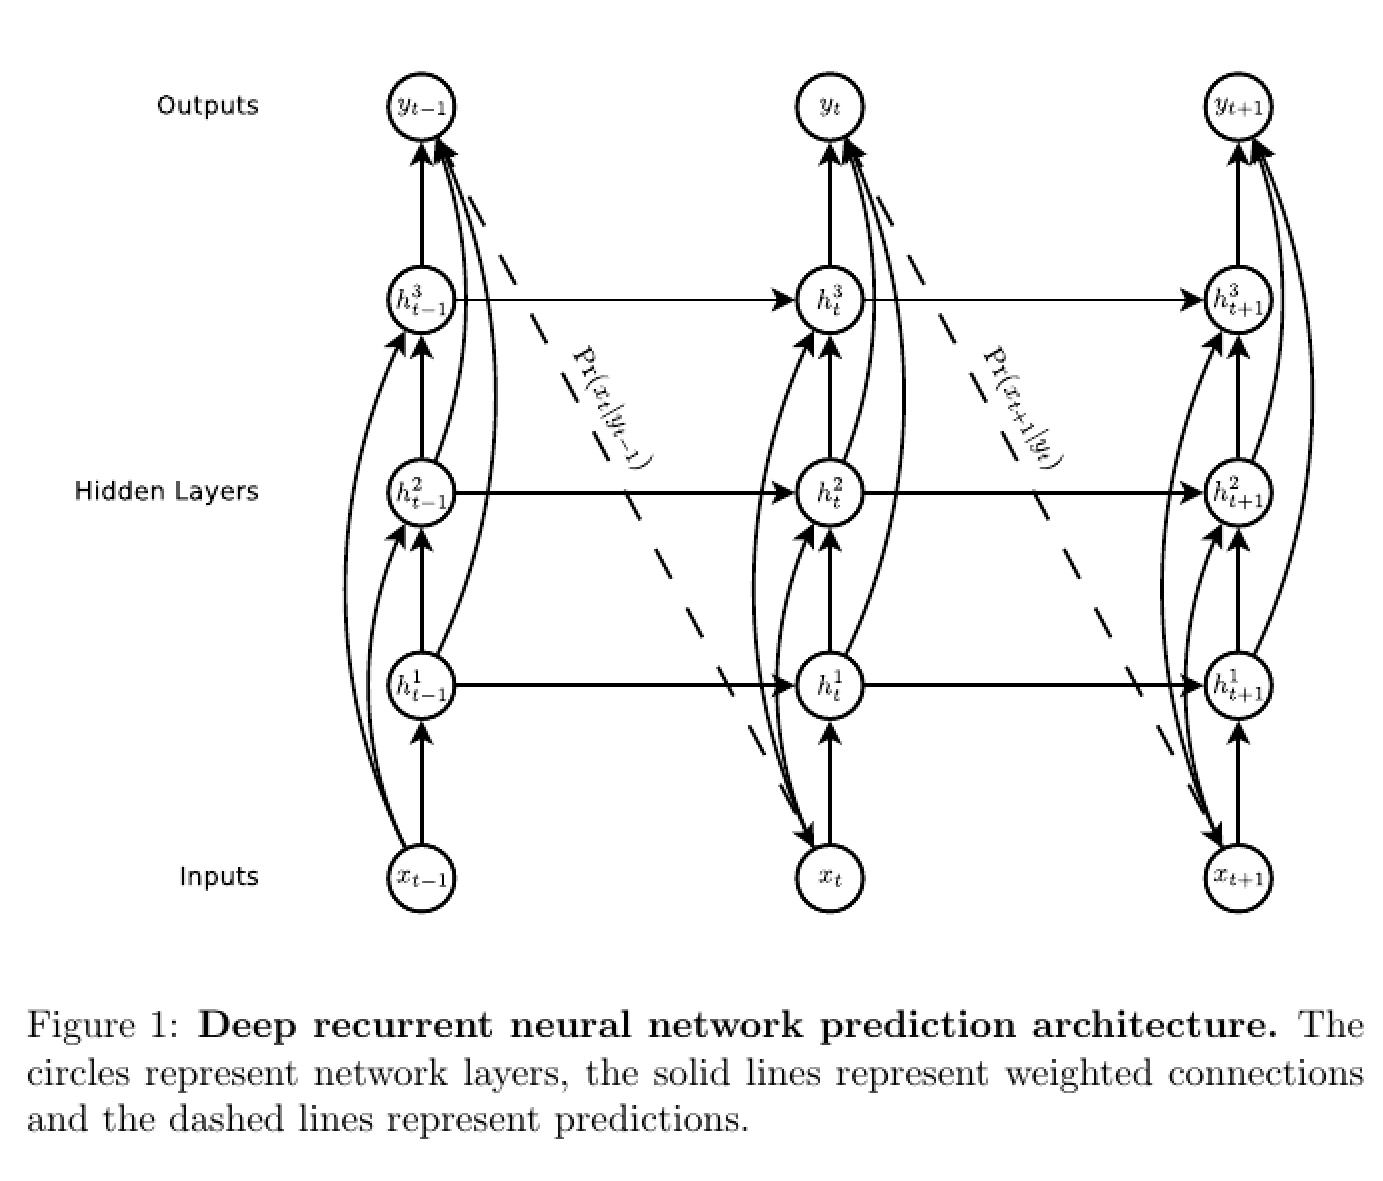
\includegraphics[width=.8\textwidth]{fig/figure1.png}
    \end{overlayarea}

    \begin{overlayarea}{\textwidth}{.3\textheight}
      \only<1>{
        Input $x_t$, hidden layers $h_t^n$, output $y_t$,
        generative model $\mathbb{P}(x_{t+1} \mid y_t)$}
  \only<2>{
    $h_t^n = $ nonlinear link $\circ$ affine combo of $x_t$, $h_{t-1}^n$, $h_t^{n-1}$
      \begin{align*}
      h_t^n = \cH(W_{ih^n} x_t + W_{h^{n-1}h^{n}} h_{t}^{n-1} + W_{h^{n}h^{n}} h_{t-1}^n + b_h^n)
      \end{align*}
  }
  \only<3>{
    $y_t =$ nonlinear link $\circ$ affine combo of $h_t^n$
    \begin{align*}
     y_t = \mathcal{Y}(b_y + \sum_{n=1}^N W_{h^n y} h_t^n)
    \end{align*}
  }
  \only<4>{
    Train by maximizing likelihood of generative model:
    \begin{align*}
     \mathbb{P}(\mathbf{x}) &= \prod_{t=1}^T \mathbb{P}(x_t \mid y_{t-1})
    \end{align*}
  }
  \only<5>{
    Compute $\nabla_\Theta \log \mathbb{P}_\Theta(\bfx)$ by "truncated backpropagation through time"
    \begin{itemize}
    \item i.e., reverse chain-rule + "clip" exploding derivatives
    \end{itemize}
  }
    \end{overlayarea}
\end{frame}


\begin{frame}{Long short term memory\footnote{graphics have slight differences
      with Graves 2013; they are taken from: \\
      \url{https://colah.github.io/posts/2015-08-Understanding-LSTMs}} }
 \begin{figure}
   \centering
   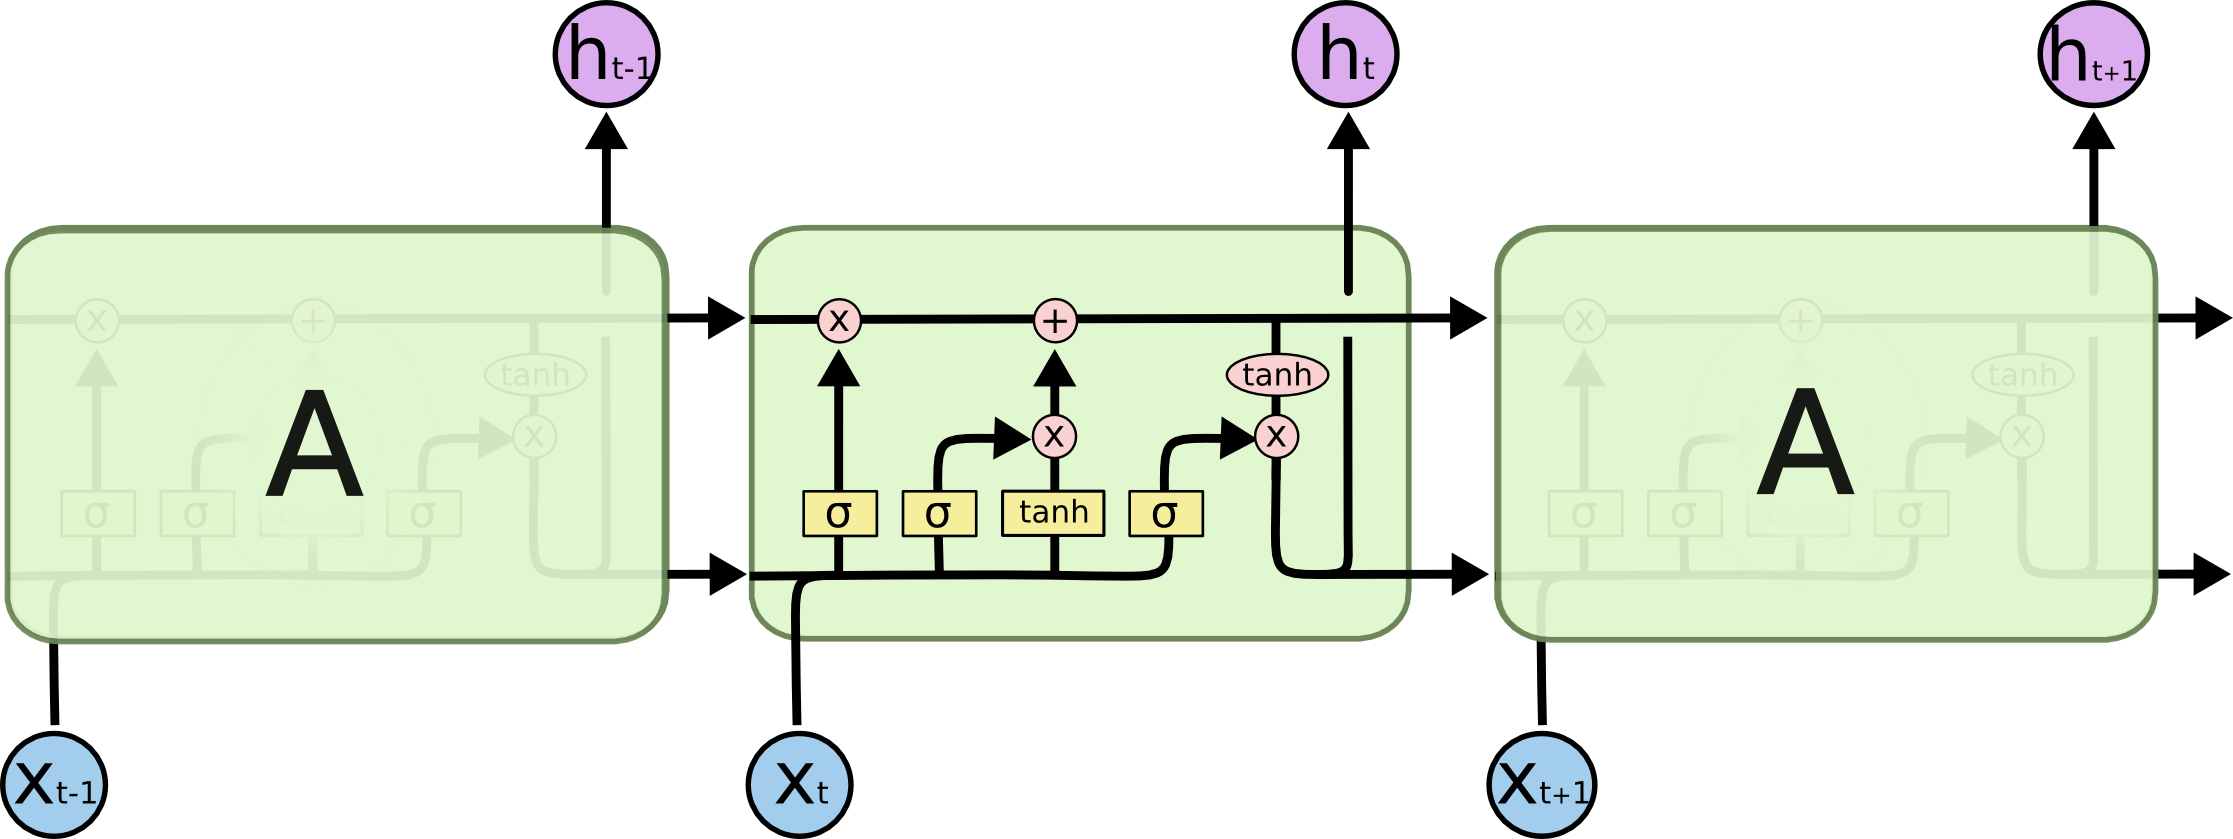
\includegraphics[width=\linewidth]{fig/LSTM3-chain.png}
 \end{figure}
\begin{columns}
  \begin{column}{.7\textwidth}
   Information passes through a series of ``gates''
   \begin{itemize}
   \item ``Gate'' = multiplication with sigmoid
     \begin{itemize}
     \item $\sigma$ = 0 $\Rightarrow$ ``let nothing thru''
     \item $\sigma$ = 1 $\Rightarrow$ ``let all thru''
     \end{itemize}
   \end{itemize}
  \end{column}

  \begin{column}{.3\textwidth}
      \begin{figure}
        %\centering
        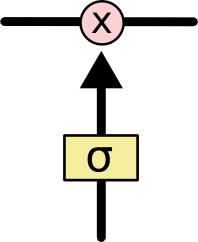
\includegraphics[width=.4\linewidth]{fig/LSTM3-gate.png}
        \label{fig:gate}
      \end{figure}
  \end{column}
\end{columns}
\end{frame}


\begin{frame}
  \begin{overlayarea}{\textwidth}{.6\textheight}
    \begin{center}
      \only<1>{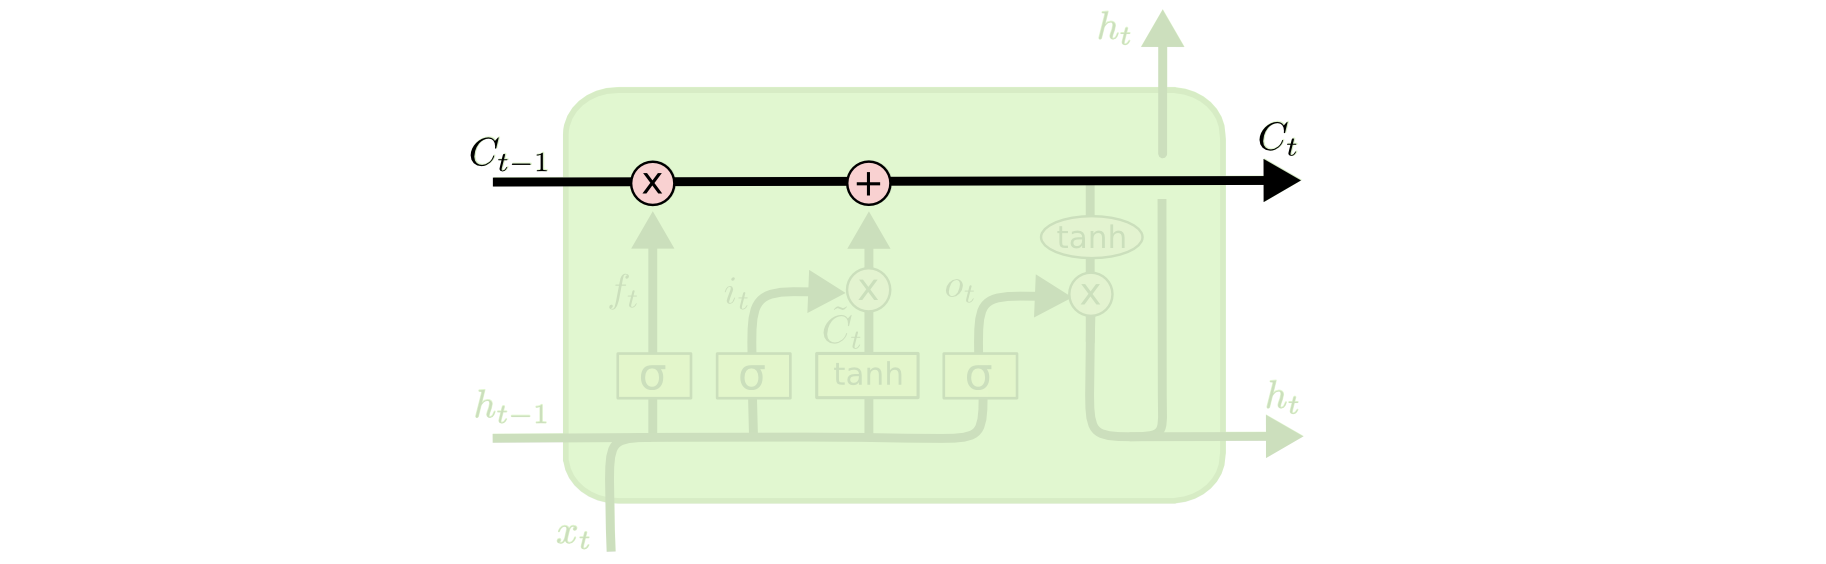
\includegraphics[width=\linewidth]{fig/LSTM3-C-line.png}}
      \only<2>{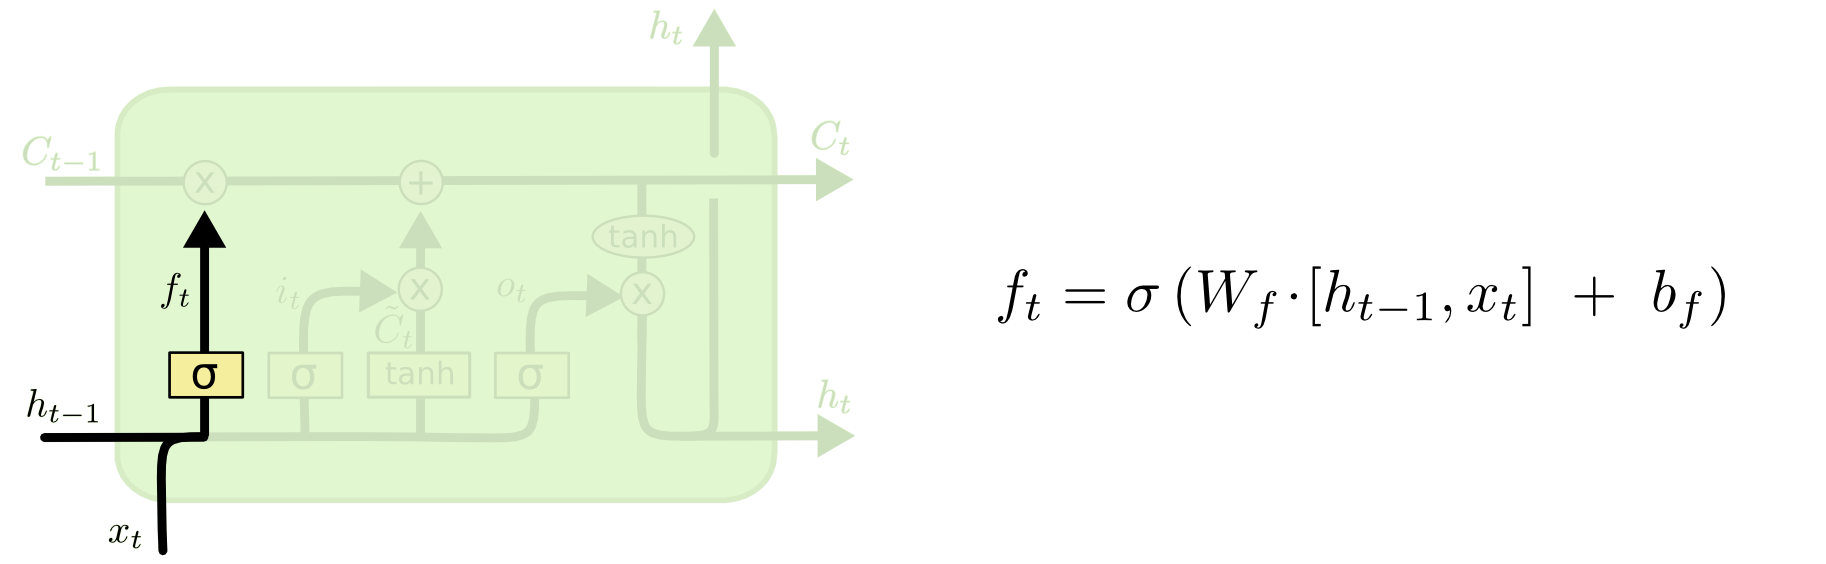
\includegraphics[width=\linewidth]{fig/LSTM3-focus-f.png}}
      \only<3>{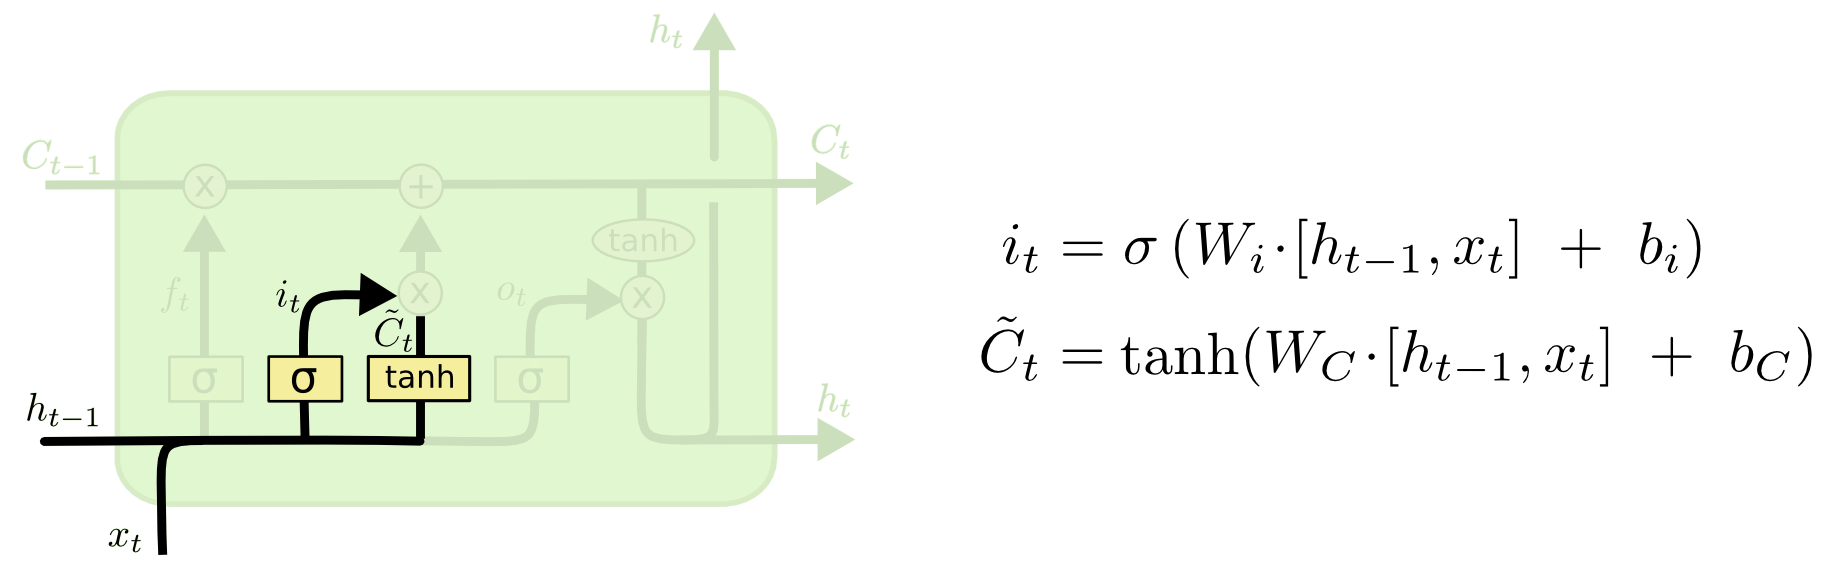
\includegraphics[width=\linewidth]{fig/LSTM3-focus-i.png}}
      \only<4>{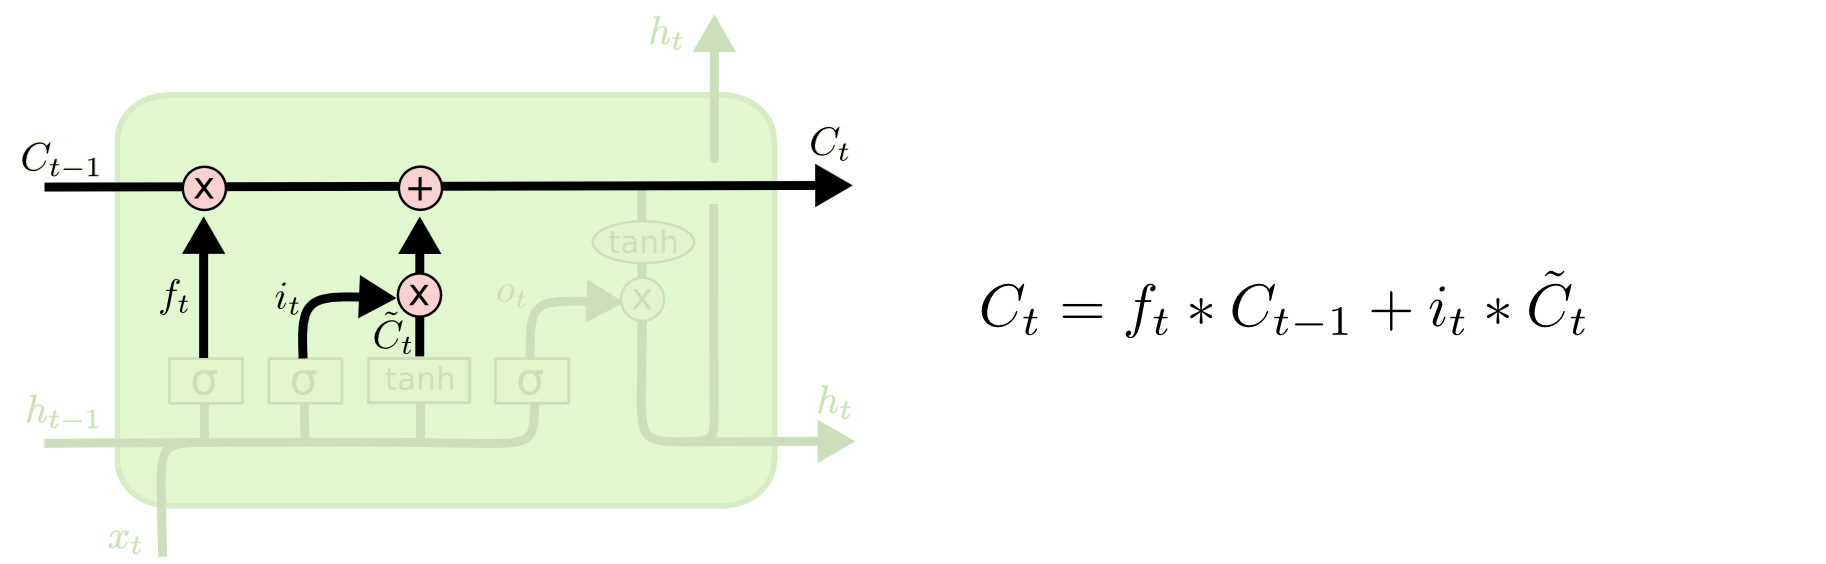
\includegraphics[width=\linewidth]{fig/LSTM3-focus-C.png}}
      \only<5>{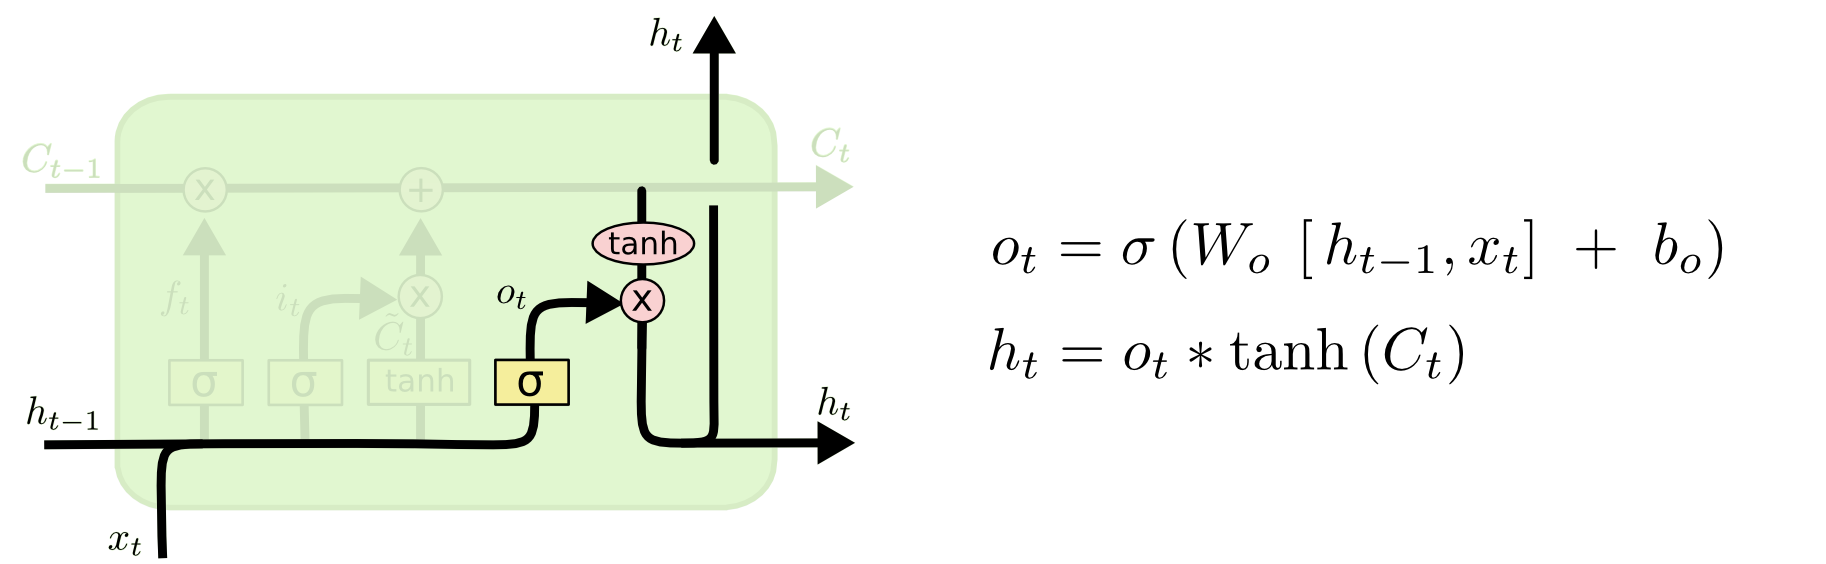
\includegraphics[width=\linewidth]{fig/LSTM3-focus-o.png}}
    \end{center}
  \end{overlayarea}
  \only<1>{$C_t$ = ``cell state'' = flows horizontally across LSTM units}
  \only<2>{$f_t$ = ``forget gate'' = gate to forget information from $C_{t-1}$}
  \only<3>{$i_t$ = ``input gate'' = gate to add information from $h_{t-1}$ and
    $x_t$ to $C_t$}
  \only<4>{Update $C_t$ using $f_t$ and $i_t$}
  \only<5>{$o_t$ = ``output gate'' = gate to output information to cell above/right}
\end{frame}

\begin{frame}{}
  Many variations on LSTM exist. Here is the one used
  in Graves 2013:
  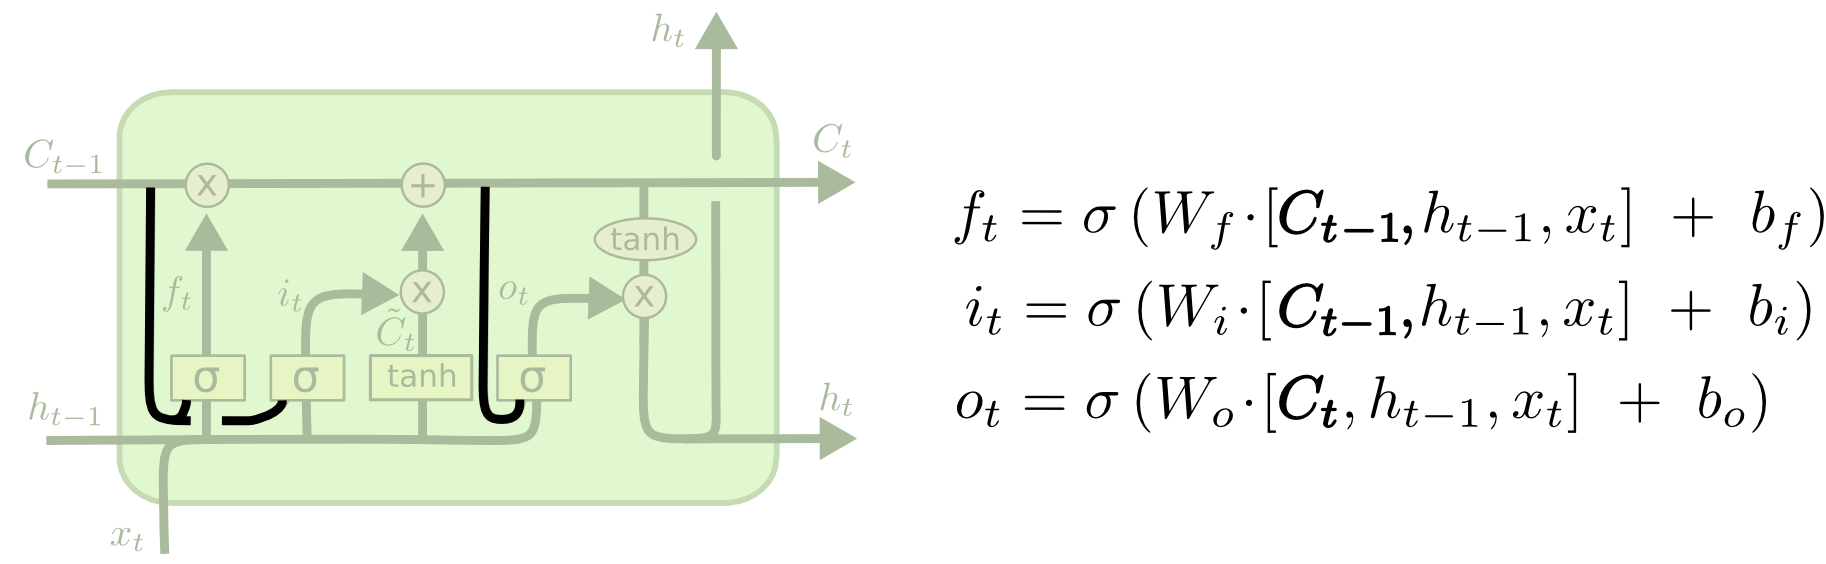
\includegraphics[width=\linewidth]{fig/LSTM3-var-peepholes.png}

  Notice the extra ``peephole'' connections from
  $C$ to $f, i, o$
\end{frame}


\section{Learning and Generating Sequences}

\begin{frame}{Text Prediction}
  How do we model a NN that takes a variable input length?
  \small{(\url{http://karpathy.github.io/2015/05/21/rnn-effectiveness/}).}
  
  \vspace{1cm}
  
  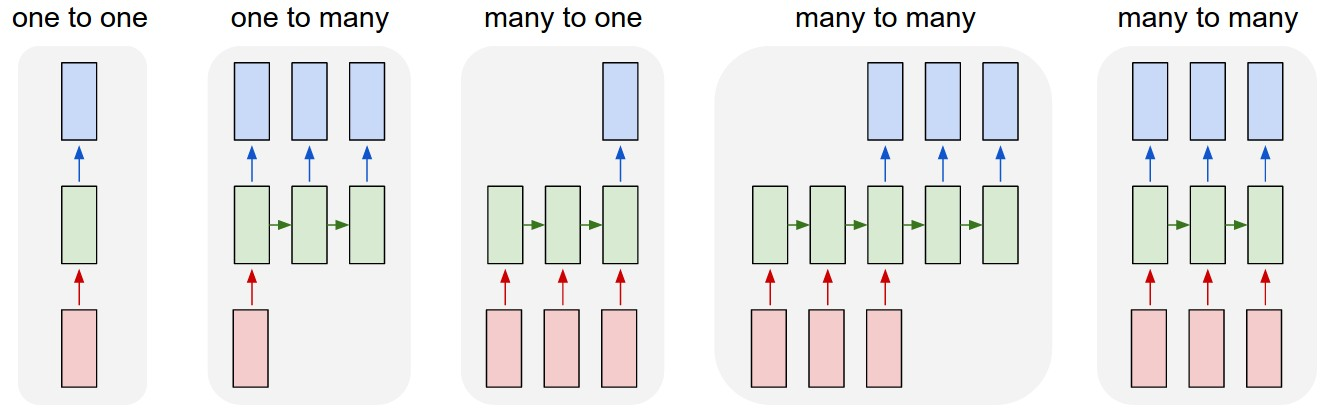
\includegraphics[width=\linewidth]{fig/nn-types.jpeg}
\end{frame}

\begin{frame}{}
  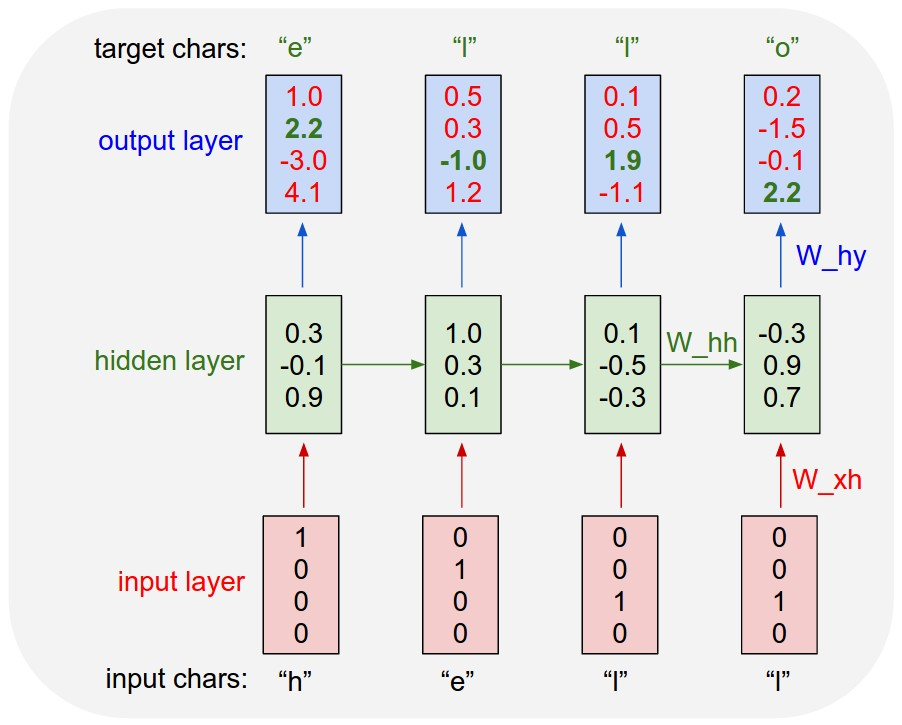
\includegraphics[width=\linewidth]{fig/nn-character.jpeg}
\end{frame}

\begin{frame}{RNN and LSTM Shakespeare}
  We compare an RNN with an LSTM to predict Shakespeare.
\end{frame}

\begin{frame}[fragile]{LSTM Shakespeare}
  \begin{lstlisting}
  KING LEAR:
  O, if you were a feeble sight, the courtesy of your law,
  Your sight and several breath, will wear the gods
  With his heads, and my hands are wonder'd at the deeds,
  So drop upon your lordship's head, and your opinion
  Shall be against your honour.
  \end{lstlisting}
\end{frame}

\begin{frame}[fragile]{LSTM Wikipedia}
  \begin{lstlisting}
 Naturalism and decision for the majority of Arab countries'
capitalide was grounded  by the Irish language by [[John
Clair]], [[An Imperial Japanese Revolt]], associated  with
Guangzham's sovereignty. His generals were the powerful
ruler of the Portugal  in the [[Protestant Immineners]],
which could be said to be directly in Cantonese 
Communication, which followed a ceremony and set inspired
prison, training. The  emperor travelled back to [[Antioch,
Perth, October 25|21]] to note, the Kingdom  of Costa Rica,
unsuccessful fashioned the [[Thrales]], [[Cynth's Dajoard]],
known  in western [[Scotland]], near Italy to the conquest
of India with the conflict. 
  \end{lstlisting}
\end{frame}

\begin{frame}[fragile]{LSTM Wiki Markdown}
  \begin{lstlisting}
  { { cite journal | id=Cerling Nonforest Department|format=Newlymeslated|none } }
  ''www.e-complete''.
  
  '''See also''': [[List of ethical consent processing]]
  
  == See also ==
  *[[Iender dome of the ED]]
  *[[Anti-autism]]
  
  ===[[Religion|Religion]]===
  *[[French Writings]]
  *[[Maria]]
  *[[Revelation]]
  *[[Mount Agamul]]
  \end{lstlisting}
\end{frame}

\begin{frame}[fragile]{LSTM XML}
  \begin{lstlisting}
<page>
  <title>Antichrist</title>
  <id>865</id>
  <revision>
    <id>15900676</id>
    <timestamp>2002-08-03T18:14:12Z</timestamp>
    <contributor>
      <username>Paris</username>
      <id>23</id>
    </contributor>
    <minor />
    <comment>Automated conversion</comment>
    <text xml:space="preserve">#REDIRECT [[Christianity]]</text>
  </revision>
</page>
  \end{lstlisting}
\end{frame}

\begin{frame}[fragile]{LSTM XML}
  \begin{lstlisting}
<page>
  <title>Antichrist</title>
  <id>865</id>
  <revision>
    <id>15900676</id>
    <timestamp>2002-08-03T18:14:12Z</timestamp>
    <contributor>
      <username>Paris</username>
      <id>23</id>
    </contributor>
    <minor />
    <comment>Automated conversion</comment>
    <text xml:space="preserve">#REDIRECT [[Christianity]]</text>
  </revision>
</page>
  \end{lstlisting}
\end{frame}

\begin{frame}{LSTM \LaTeX}
  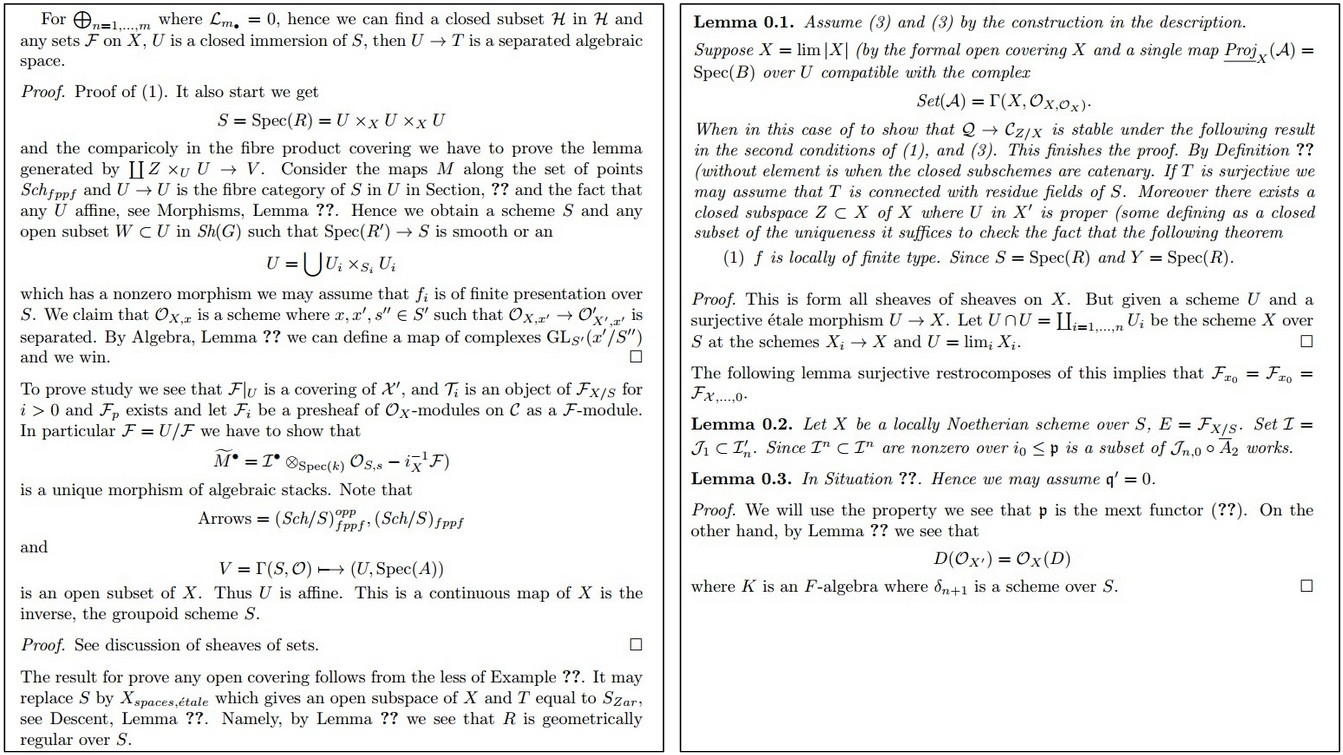
\includegraphics[width=\linewidth]{fig/lstm-latex-1.jpeg}
\end{frame}

\begin{frame}[fragile]{LSTM C++}
\begin{lstlisting}
/*
 * If this error is set, we will need anything right after
 * that BSD.
 */
static void action_new_function(struct s_stat_info *wb)
{
  unsigned long flags;
  int lel_idx_bit = e->edd, *sys & ~((unsigned long) *FIRST_COMPAT);
  buf[0] = 0xFFFFFFFF & (bit << 4);
  min(inc, slist->bytes);
  printk(KERN_WARNING "Memory allocated %02x/%02x, "
    "original MLL instead\n"),
    min(min(multi_run - s->len, max) * num_data_in),
    frame_pos, sz + first_seg);
  div_u64_w(val, inb_p);
  spin_unlock(&disk->queue_lock);
  mutex_unlock(&s->sock->mutex);
  mutex_unlock(&func->mutex);
  return disassemble(info->pending_bh);
}
\end{lstlisting}
\end{frame}

\begin{frame}[fragile]{LSTM C++}

\begin{lstlisting}[basicstyle=\tiny\ttfamily]
static void num_serial_settings(struct tty_struct *tty)
{
  if (tty == tty)
    disable_single_st_p(dev);
  pci_disable_spool(port);
  return 0;
}

static void do_command(struct seq_file *m, void *v)
{
  int column = 32 << (cmd[2] & 0x80);
  if (state)
    cmd = (int)(int_state ^ (in_8(&ch->ch_flags) & Cmd) ? 2 : 1);
  else
    seq = 1;
  for (i = 0; i < 16; i++) {
    if (k & (1 << 1))
      pipe = (in_use & UMXTHREAD_UNCCA) +
        ((count & 0x00000000fffffff8) & 0x000000f) << 8;
    if (count == 0)
      sub(pid, ppc_md.kexec_handle, 0x20000000);
    pipe_set_bytes(i, 0);
  }
  /* Free our user pages pointer to place camera if all dash */
  subsystem_info = &of_changes[PAGE_SIZE];
  rek_controls(offset, idx, &soffset);
  /* Now we want to deliberately put it to device */
  control_check_polarity(&context, val, 0);
  for (i = 0; i < COUNTER; i++)
    seq_puts(s, "policy ");
}
\end{lstlisting}
\end{frame}

\begin{frame}{Visualizing Predictions: What Do Neurons Do?}
  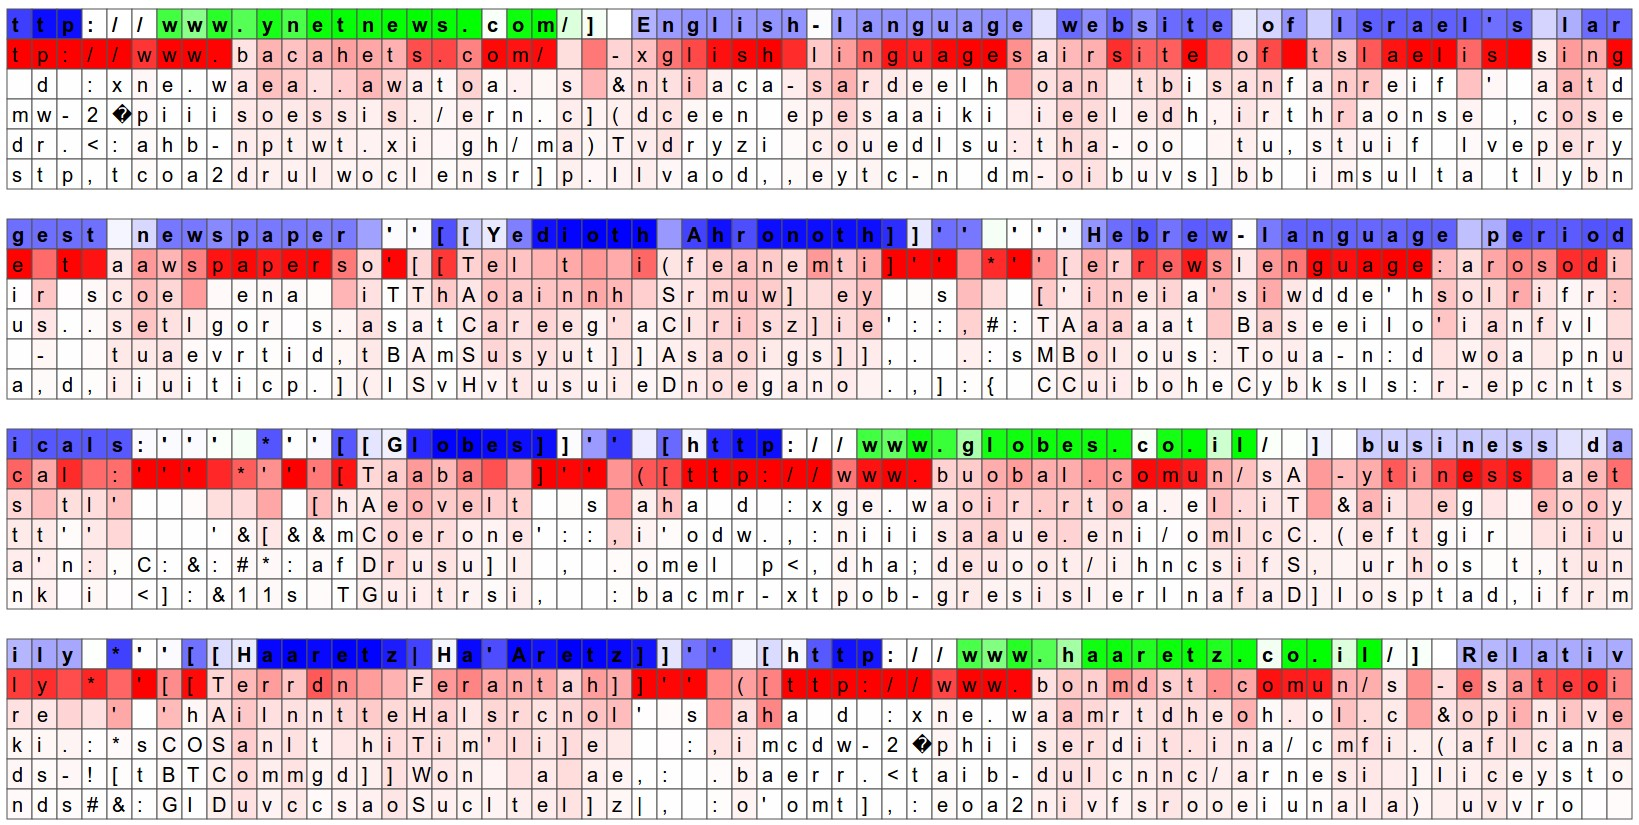
\includegraphics[width=\linewidth]{fig/lstm-pred-1.jpeg}
\end{frame}
\begin{frame}{Visualizing Predictions: What Do Neurons Do?}
  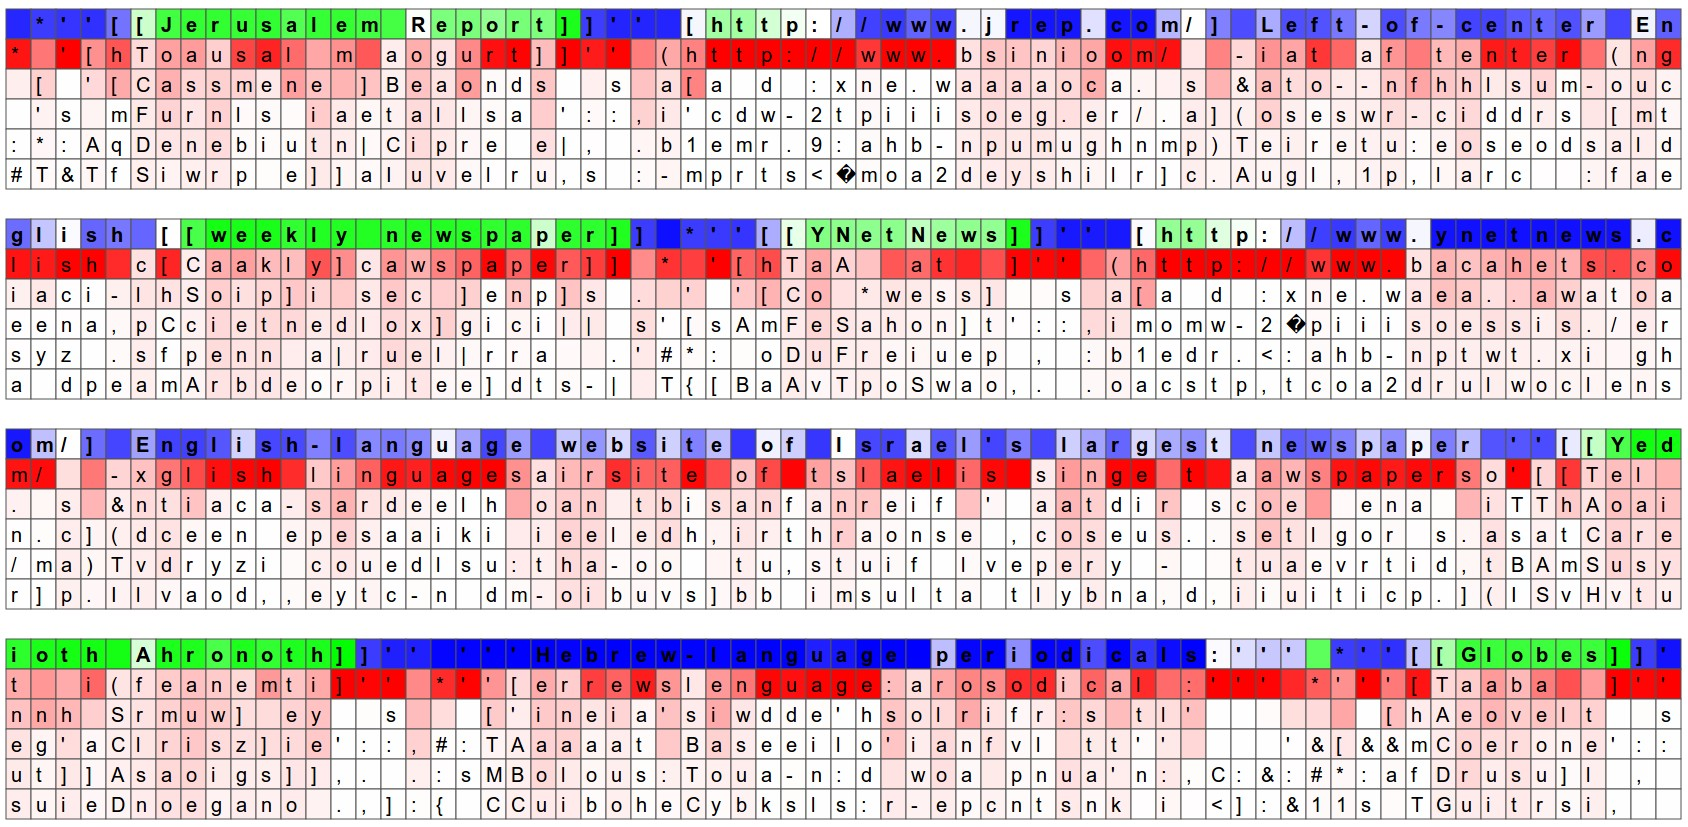
\includegraphics[width=\linewidth]{fig/lstm-pred-2.jpeg}
\end{frame}
\begin{frame}{Visualizing Predictions: What Do Neurons Do?}
  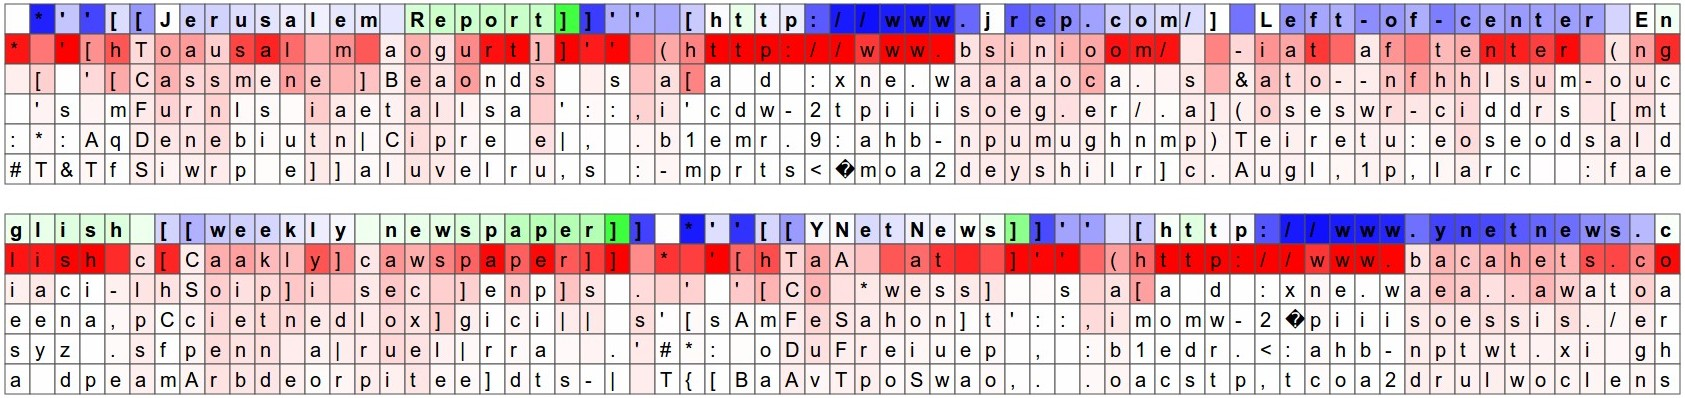
\includegraphics[width=\linewidth]{fig/lstm-pred-3.jpeg}
\end{frame}
\begin{frame}{Visualizing Predictions: What Do Neurons Do?}
  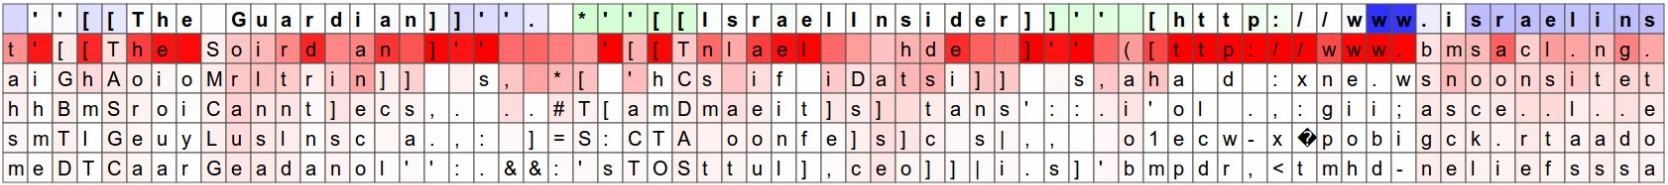
\includegraphics[width=\linewidth]{fig/lstm-pred-4.jpeg}
\end{frame}
\begin{frame}{Visualizing Predictions: What Do Neurons Do?}
  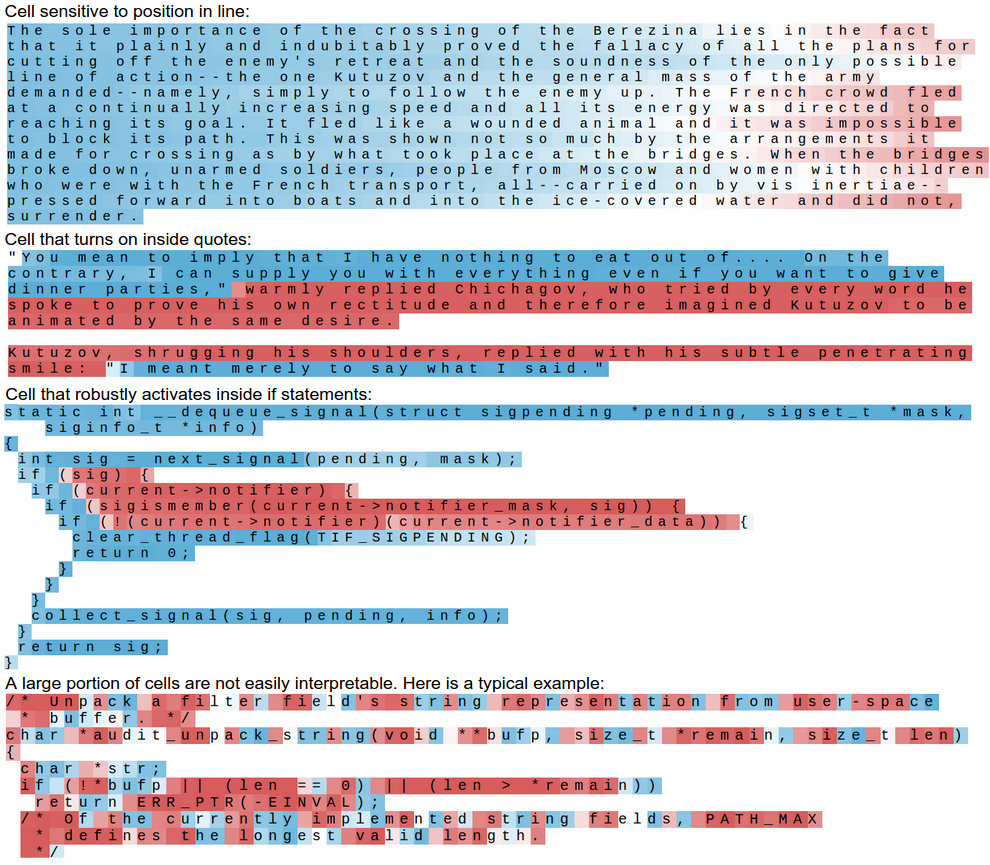
\includegraphics[width=\linewidth,trim=0 17cm 0 0,clip]{fig/lstm-pred-5.png}
\end{frame}
\begin{frame}{Visualizing Predictions: What Do Neurons Do?}
  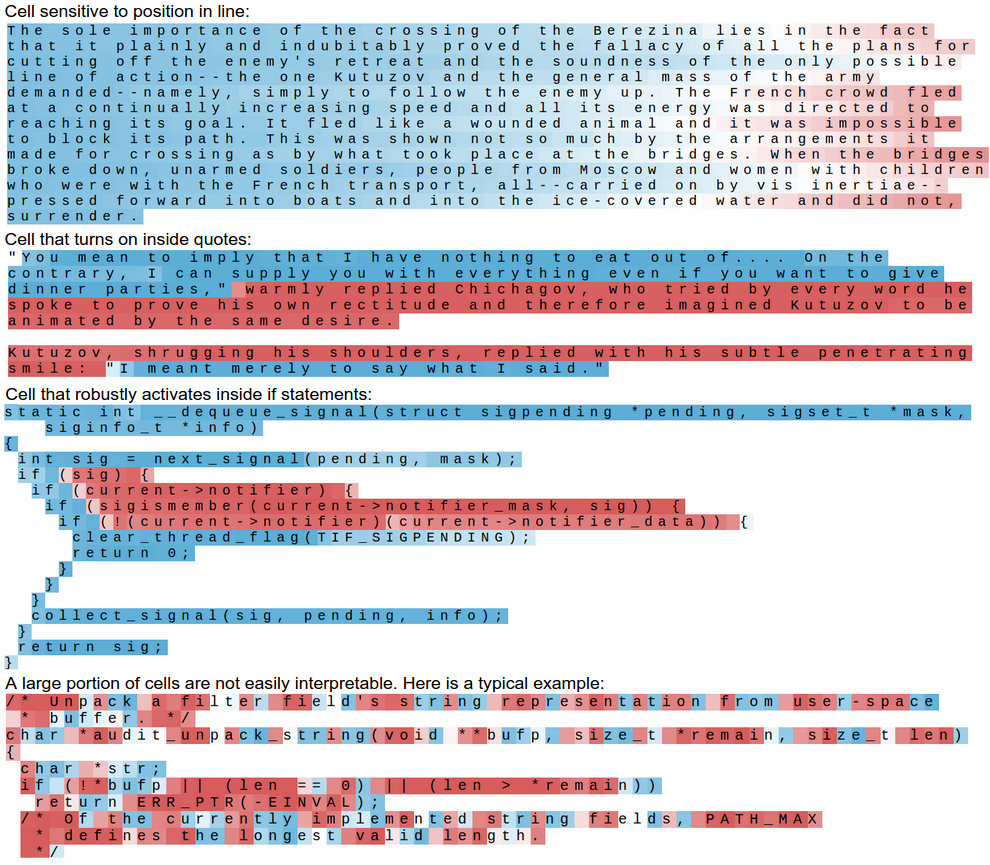
\includegraphics[width=\linewidth,trim=0 0 0 13.5cm,clip]{fig/lstm-pred-5.png}
\end{frame}
\begin{frame}{Visualizing Predictions: What Do Neurons Do?}
  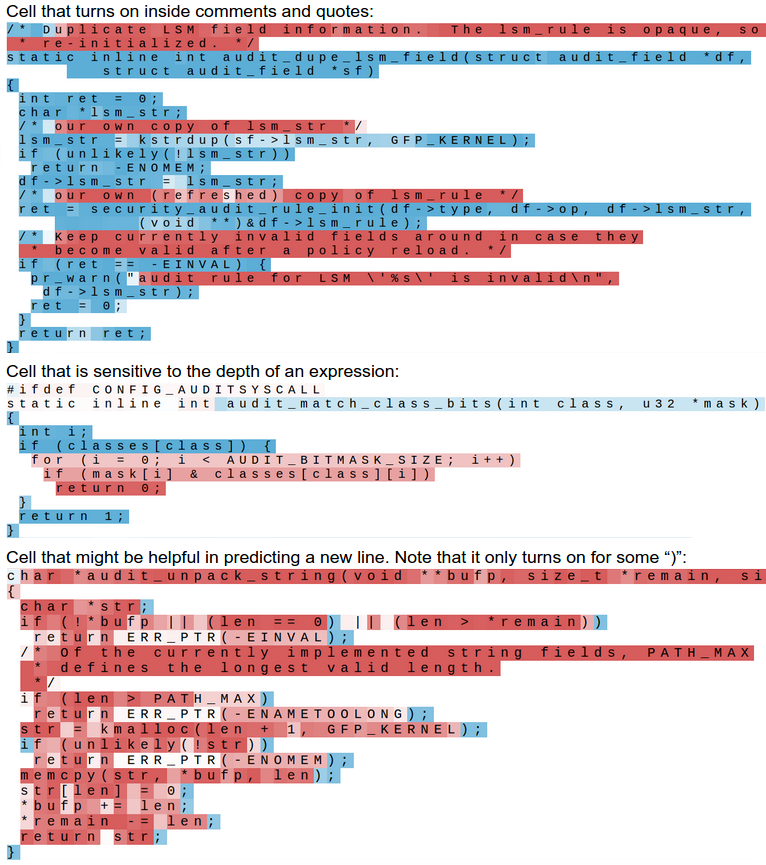
\includegraphics[width=\linewidth,trim=0 18cm 0 0,clip]{fig/lstm-pred-6.png}
\end{frame}
\begin{frame}{Visualizing Predictions: What Do Neurons Do?}
  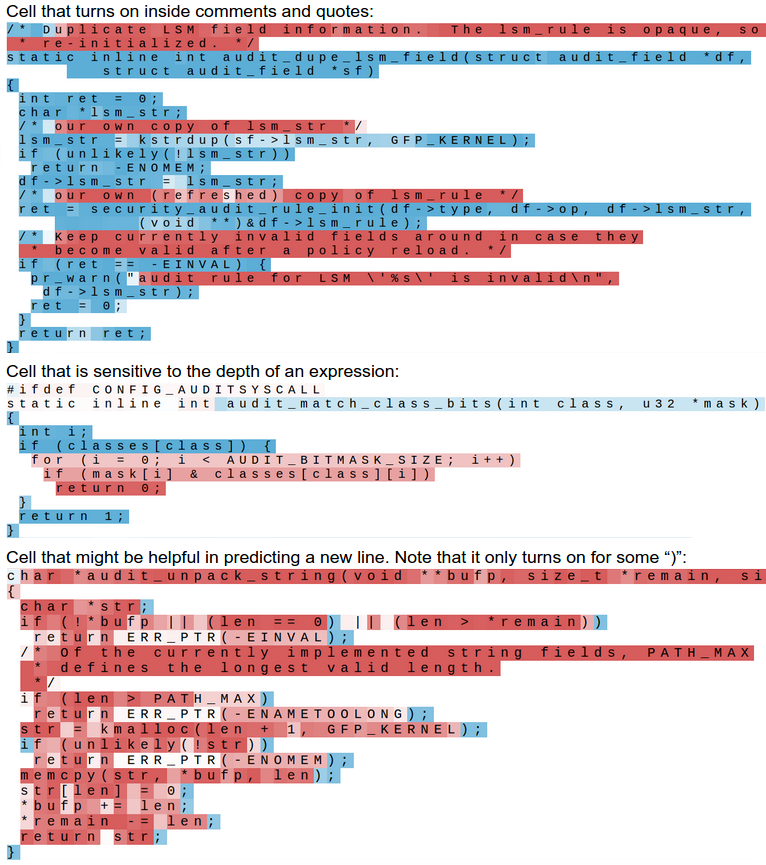
\includegraphics[width=\linewidth,trim=0 0 0 12.7cm,clip]{fig/lstm-pred-6.png}
\end{frame}

\section{Generating handwriting}
\begin{frame}
  \begin{figure}
    \centering
  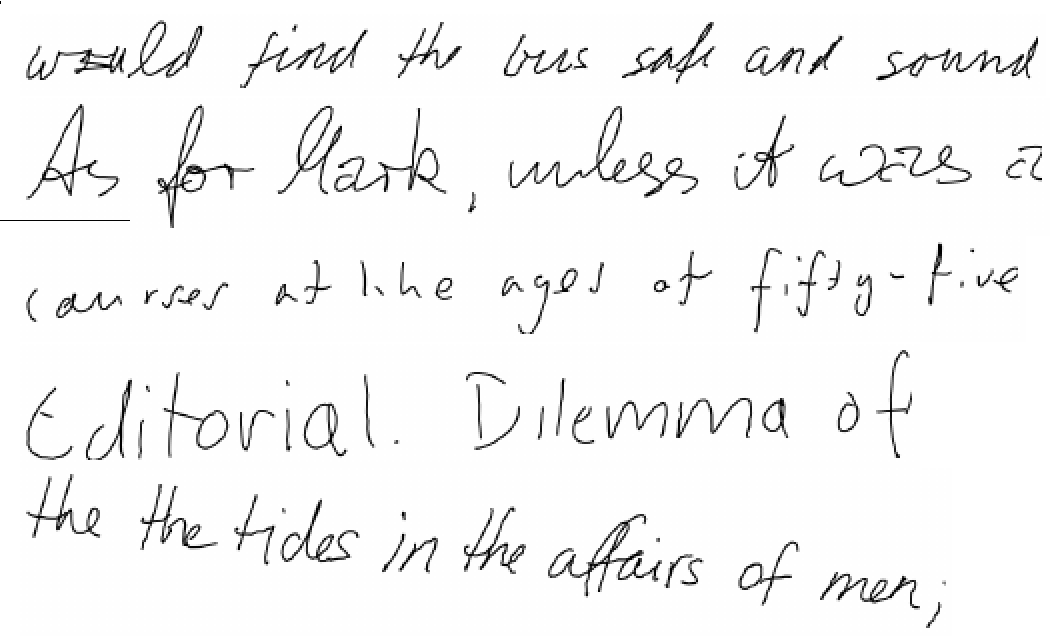
\includegraphics[width=.75\linewidth]{fig/fig9.png}
    \caption{Training samples from IAM handwriting database}
    \label{fig:fig9}
  \end{figure}
Input $x_t$ = ($\texttt{pos}_t - \texttt{pos}_{t-1}$) $\times$
(is-end-of-stroke) $ \in \mathbb{R}^2 \times \{0,1\}$
\end{frame}

\begin{frame}
  \frametitle{Mixture density network}
  \begin{align*}
   x_t &\in \mathbb{R} \times \mathbb{R} \times \{0,1\}  \\
    y_t &= (e_t, \{\pi^j_t, \mu^j_t, \sigma^j_t, \rho^j_t\}_{j=1}^M) \\
    \mathbb{P}(x_{t+1} \mid y_t) &= \sum_{j=1}^M \pi^j_t \mathcal{N}(x_{t+1} \mid \mu^j_t, \sigma^j_t, \rho^j_t)
    \begin{cases}
      e_t & \text{if } (x_{t+1})_3 = 1 \\
      1-e_t & \text{else}
    \end{cases}
  \end{align*}

  \begin{itemize}
  \item $e_t$ = end-of-stroke prob = $\frac1{1+\exp(\hat{e}_t)}$
  \item $\pi^j_t$ = mixture prob $= \frac{\exp(\hat{\pi}_t^j)}{\sum_{j'}\exp(\hat{\pi}_t^{j'})}$
  \item $\mu^j_t$ = component mean $= \hat{\mu}^j_t$
  \item $\sigma^j_t$ = component variance $= \exp(\hat{\sigma}_t^j)$
  \item $\rho^j_t$ = component x/y correlation $= \text{tanh}(\hat{\rho}^j_t)$
  \end{itemize}
\end{frame}

\begin{frame}
  \begin{figure}
    \centering
    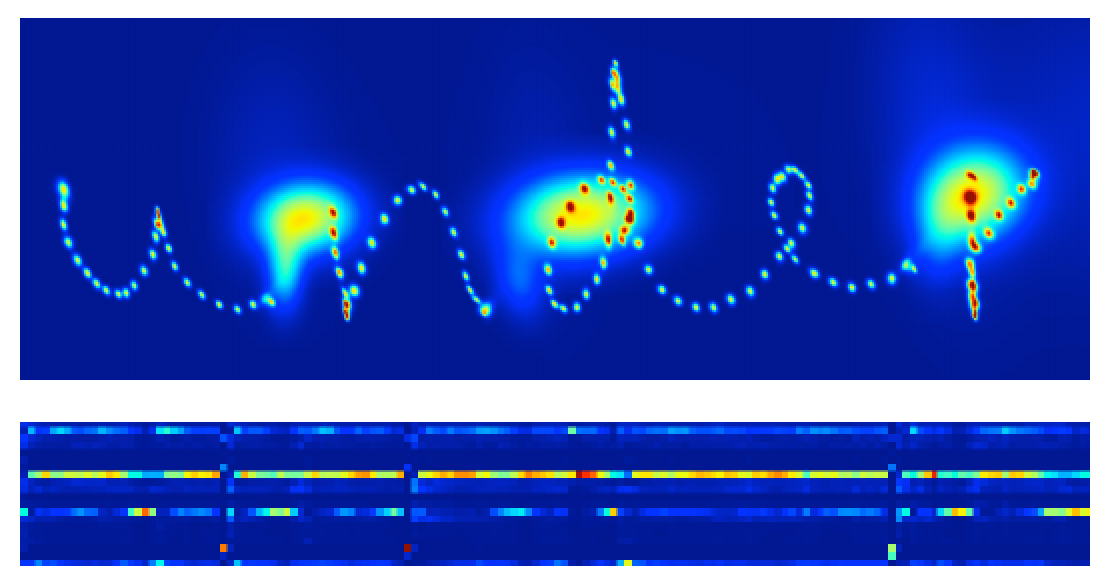
\includegraphics[width=.75\linewidth]{fig/fig10.png}
    \caption{Mixture density outputs as word ``under'' is written}
    \label{fig:fig10}
  \end{figure}
  \begin{itemize}
  \item Blobs = Predictions at end of strokes for first point in next stroke
  \item Lower panel = component weights
  \end{itemize}
\end{frame}

\begin{frame}
\begin{columns}
  \begin{column}{.5\textwidth}
  \begin{figure}
    \centering
    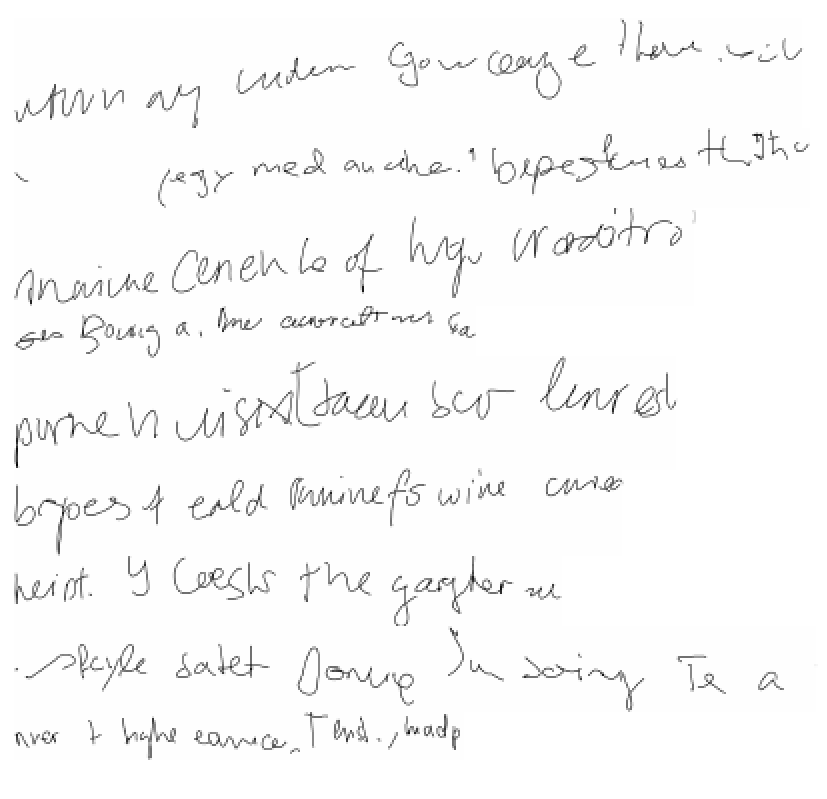
\includegraphics[width=\linewidth]{fig/fig11.png}
    \caption{Samples generated by prediction network (700-timesteps each).
      Network has learned strokes, some characters, and even short words (e.g. ``of'').}
    \label{fig:fig11}
  \end{figure}
  \end{column}

  \begin{column}{.5\textwidth}
    \begin{itemize}
    \item 3 hidden layers, each with 400 LSTM cells
    \item $3.4 \times 10^6$ parameters total
    \item Trained with rmsprop and adaptive weight noise
    \item Output derivatives $\frac{\partial \log
        \mathbb{P}(\mathbf{x})}{\partial \hat{y}_t}$ clipped to be in $[-100,
      100]$; LSTM derivatives clipped within $[-10, 10]$
      \begin{itemize}
      \item Clipping vital for numerical stability
      \end{itemize}
    \end{itemize}
  \end{column}
\end{columns}
\end{frame}

\begin{frame}
  \frametitle{Handwriting synthesis}
  \begin{itemize}
  \item Generate handwriting for a given text
  \item Main challenge: aligning continuous handwriting sequence with discrete text
  \item Main idea: bottom hidden layer maintains a distribution of the current position
    in the text (``soft window'')
  \end{itemize}
\end{frame}

\begin{frame}{Synthesis Network}
  \begin{figure}
    \centering
  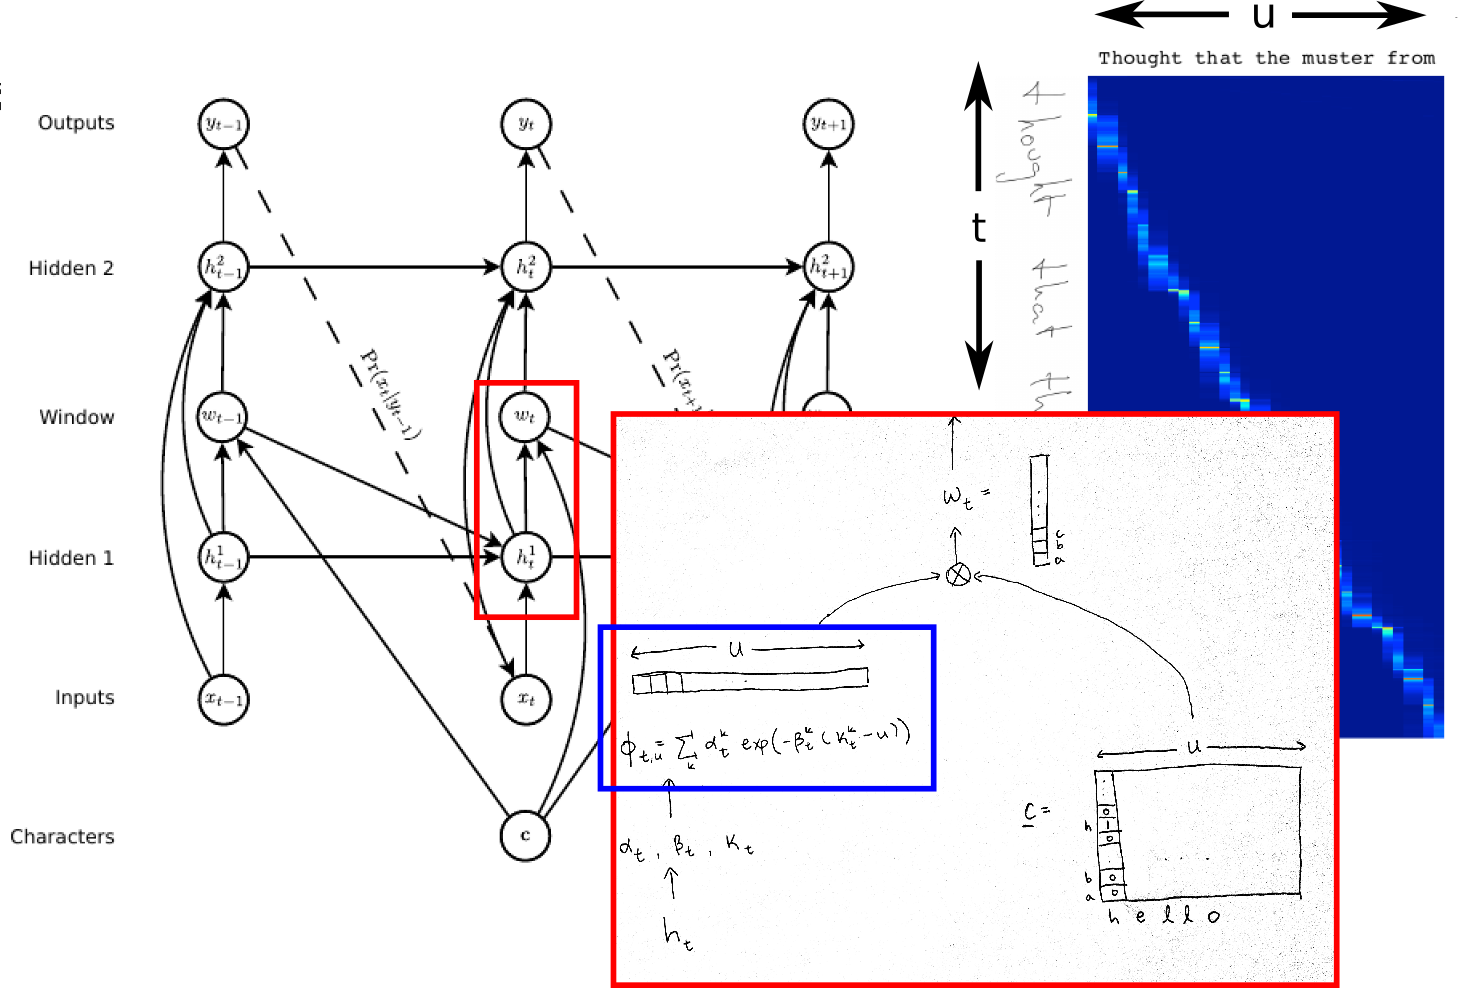
\includegraphics[width=.9\linewidth]{fig/synthesis_network3.png}
    \caption{$\phi_t(h_t^1) = $ distn over positions; $w_t = \mathbf{c}
      \phi_t =$ distn over characters}
    \label{fig:synthesis-network}
  \end{figure}
\end{frame}

\begin{frame}
  \frametitle{Unbiased sampling}
 \begin{columns}
   \begin{column}{.5\textwidth}
     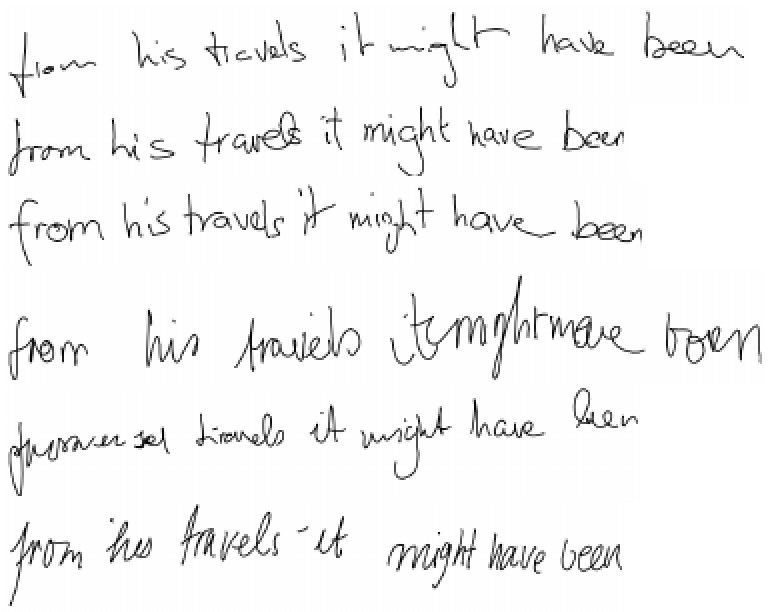
\includegraphics[width=\linewidth]{fig/fig15a.png}
   \end{column}

   \begin{column}{.5\textwidth}
     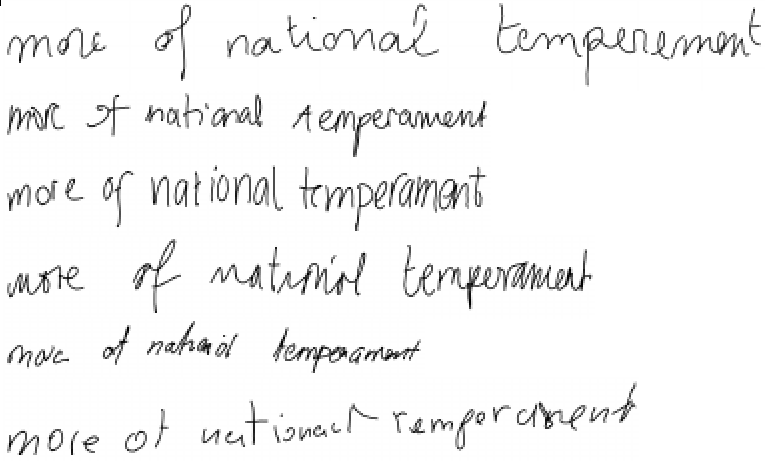
\includegraphics[width=\linewidth]{fig/fig15b.png}
   \end{column}
 \end{columns} 
 \begin{itemize}
 \item Sample from $\mathbb{P}(\bfx \mid \bfc)$ by iteratively sampling from
   $\bbP(x_{t+1} \mid y_t)$
 \item Stop when $\phi(t, U+1) > \max_{u \leq U} \phi(t, u)$ 
 \item First line of each block is real; subsequent lines generated by network
 \end{itemize}
\end{frame}

\begin{frame}
  \frametitle{Biased sampling}
\begin{columns}
  \begin{column}{.5\textwidth}
    \begin{figure}
      \centering
  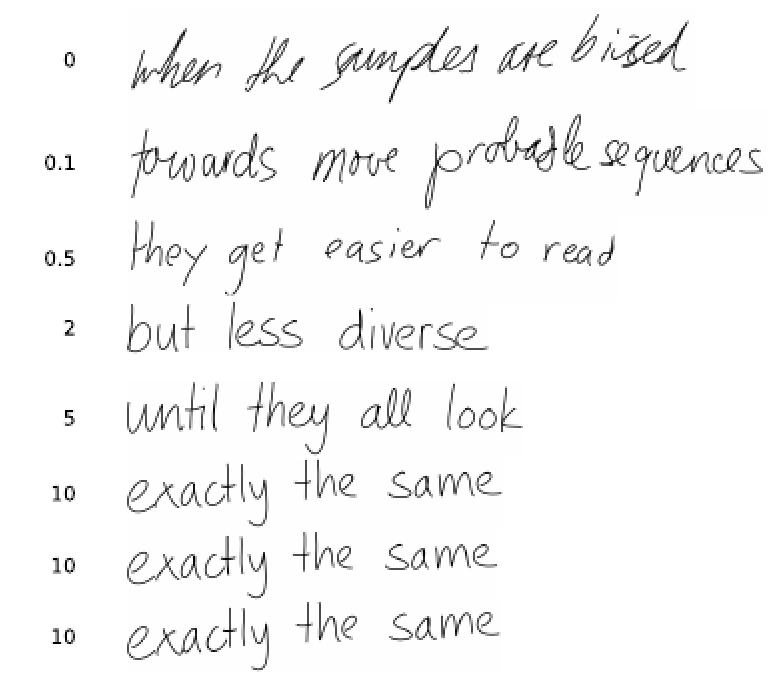
\includegraphics[width=\linewidth]{fig/fig16.png}
      \caption{what is the bias term mean here}
      \label{fig:fig16}
    \end{figure}
  \end{column}

  \begin{column}{.5\textwidth}
    \begin{itemize}
    \item Decreasing the variance of the output sequences leads to neater handwriting
    \end{itemize}
  \end{column}
\end{columns}
\end{frame}

\begin{frame}
  \frametitle{Primed sampling}
  
\end{frame}

\end{document}
